\chapter{Оценка матрицы разброса}

В предыдущих главах рассматривались робастные методы оценивания многомерного параметра положения. Однако во многих задачах многомерного анализа требуется также робастная оценка матрицы разброса.

\section{Метод оценивания вдоль случайных направлений}

Для робастной оценки матрицы разброса $\mathbf{S} \in \mathbb{R}^{d \times d}$ воспользуемся идеей, применявшейся ранее в методах, основанных на алгоритмах концентрации (см. раздел~\ref{sec:concentration}). Модифицируем Алгоритм~\ref{alg:median} таким образом, чтобы на каждой итерации вместе с оценкой медианы вычислялось также медианное абсолютное отклонение ($\mathrm{MAD}$) вдоль выбранного направления.

В отличие от методов концентрации, здесь не используется процедура отбрасывания части выборки. Вместо этого информация о разбросе данных извлекается из проекций выборки на случайные направления.

\textbf{Идея метода}

Известно, что проекция многомерной случайной величины с ковариационной матрицей $\boldsymbol{\Sigma}$ на направление $\mathbf{u}$ имеет дисперсию $\sigma^2 = \sigma^2_{\mathbf{u}} = \mathbf{u}^{\mathrm{T}} \boldsymbol{\Sigma} \mathbf{u}$.

В общем случае заменим матрицу $\boldsymbol{\Sigma}$  на $\mathbf{S}$, а $\sigma^2_{\mathbf{u}}$ на
\begin{equation}\label{eq:mad}
    \widehat{\text{MAD}}^2_{\mathbf{u}} = \left(\frac{1}{\Phi^{-1}(3/4)} \text{MAD}_{\mathbf{u}}\right)^2,
\end{equation}
где $\Phi$ ---  функция распределения стандартной нормальной величины. Коэффициент $\Phi^{-1}(3/4)$ возникает из известного соотношения между MAD и среднеквадратическим отклонением для нормального распределения.

Таким образом, вводится нормировка, чтобы в случае нормального распределения матрица разброса сходилась к ковариационной матрице с ростом размера выборки. 

Пусть на $i$-й итерации Алгоритма~\ref{alg:median} выбрано случайное направление $\mathbf{u}_i$. Для него вычислим величину $\widehat{\mathrm{MAD}}_{\mathbf{u}_i}^2$. По аналогии с нормальной моделью будем считать, что выполняется приближенное соотношение
\begin{equation}\label{eq_mad}
    \widehat{\mathrm{MAD}}_{\mathbf{u}_i}^2
    \approx
    \mathbf{u}^{\mathrm{T}}_i\mathbf{S}\mathbf{u}_i.
\end{equation}

Тогда задача оценки матрицы $\mathbf{S}$ сводится к оценке её элементов, используя соотношение \eqref{eq_mad}.

Поскольку матрица $\mathbf{S}$ симметрична, достаточно оценивать только элементы верхнего треугольника $s_{11}$, \ldots, $s_{ij}$, \ldots, $s_{dd}$, $i \leqslant j$. 
Общее число неизвестных параметров равно $r = \frac{d(d+1)}{2}$.

Пусть $\mathbf{u}_i = (u_1^i, \ldots, u_d^i)^\rmT$. Тогда выражение $\mathbf{u}_i^{\mathrm{T}}\mathbf{S}\mathbf{u}_i$
является линейной комбинацией элементов матрицы $\mathbf{S}$:
% Тогда $\mathbf{u}_i^\rmT \mathbf{S} \mathbf{u}_i$ для $i = 1, \ldots, k$ (где $k$ --- общее число итераций Алгоритма~\ref{alg:median}) являются линейными
% комбинациями элементов $s_{i, j}$. Пусть $\mathbf{u}_i = (u_1^i, \ldots, u_d^i)^\rmT$, тогда верно следующее:
\begin{equation}\label{eq:linearform}
    \mathbf{u}_i^\rmT \mathbf{S} \mathbf{u}_i = \sum_{j = 1}^d (u_j^i)^2 s_{jj} + \sum_{1 \leqslant j < p \leqslant d} 2 u_j^i u_p^i s_{jp},
\end{equation}
где $i = 1, \ldots, K$, а $K$ --- общее число итераций Алгоритма~\ref{alg:median}.

Следовательно, используя несколько случайных направлений, можно получить систему линейных уравнений относительно неизвестных коэффициентов~$s_{ij}$.

Для каждого направления $\mathbf{u}_i$ сформируем строку матрицы регрессоров $\hat{\mathbf{X}}\in \mathbb{R}^{K \times r}$ из коэффициентов $(u_j^i)^2$ и $u_j^i u_p^i$ перед элементами $s_{ij}$ в выражении~\eqref{eq:linearform}. Соответствующие значения $\widehat{\mathrm{MAD}}_{\mathbf{u}_i}^2$ образуют вектор $\mathbf{z} \in \mathbb{R}^K$.

% Следовательно, если для каждого $i$ взять коэффициенты $(u_j^i)^2$ и $u_j^i u_k^i$ перед элементами $s_{i, j}$ из \eqref{eq:linearform}, всего $r$ штук, и составить из них матрицу регрессоров $\mathbf{X} \in \mathbb{R}^{k \times r}$, а элементы из $\widehat{\text{MAD}}^2_{\mathbf{u}_i}$ положить в вектор $\mathbf{y} \in \mathbb{R}^k$,
% то используя выражение \eqref{eq_mad} для $i = 1, \ldots, k$  можем оценить коэффициенты $s_{i, j}$, $1 \le i \le j \le d$ (назовём
% эти оценки $\hat{\mathbf{s}} = (\hat s_{i, j})$, используя обычный линейный МНК для матрицы-регрессора $\mathbf{X}$ и зависимого вектора $\mathbf{y}$: $\hat{\mathbf{s}} = \mathbf{X}^- \mathbf{y},$ где $\mathbf{X}^-$ --- псевдообратная Мура-Пенроуза к $\mathbf{X}$.


Тогда задача оценки матрицы разброса сводится к линейной регрессии:
\begin{equation*}
\widehat{\mathbf{s}} = \hat{\mathbf{X}}^{-}\mathbf{z},
\end{equation*}
где $\hat{\mathbf{X}}^{-}$ --- псевдообратная матрица Мура--Пенроуза, а $\widehat{\mathbf{s}}=(\widehat{s}_{ij})$ --- оценки элементов матрицы разброса.

Таким образом, оценивание матрицы разброса сводится к восстановлению коэффициентов линейной системы, построенной по случайным направлениям и робастным оценкам масштаба вдоль этих направлений. Полученный метод представлен в виде Алгоритма~\ref{alg:dispercematrix_naive}.

Заметим, что минимально требующееся количество итераций $K$ для Алгоритма~\ref{alg:median} равно $r$, иначе выборка направлений будет недостаточной по размеру для построения оценки $\widehat{\mathbf{S}}$.

Кроме того, алгоритм эквивариантен относительно случайных поворотов, так как использует случайно выбранные направления для оценки MAD.

% Основная проблема Алгоритма~\ref{alg:dispercematrix_naive} состоит в том, что очень тяжело контролировать вырожденность и обусловленность матрицы $\mathbf{X}$ --- вообще говоря, её число обусловленности случайно. В связи с этим уже для достаточно малых $d$ может наблюдаться неустойчивость в его работе.

Несмотря на естественность данной конструкции, Алгоритм~\ref{alg:dispercematrix_naive} обладает существенным недостатком. Матрица регрессоров $\hat{\mathbf{X}}$ строится на основе случайных направлений, поэтому ее число обусловленности также является случайной величиной. В результате система может оказаться плохо обусловленной или даже близкой к вырожденной, что приводит к численной неустойчивости оценки.

Именно эта проблема делает прямое восстановление матрицы разброса по случайным направлениям практически неприменимым в пространствах высокой  размерности.


\begin{algorithm}[H]
\caption{Наивное вычисление оценки матрицы разброса вдоль случайных направлений}
\begin{algorithmic}[1]
			\State Рассматриваем выборку $\mathbf{x}_1,\ldots,\mathbf{x}_{{n}}$. 
			\State Задаём $i=1$ --- первый шаг алгоритма, $K$ --- общее число шагов, $K \geqslant r$. 
			\State Рассматриваем случайный вектор $\mathbf{u}_i$, равномерно распределенный на единичной сфере. Проводим прямую  $l_i=\{\lambda\mathbf{u}_{{i}},\;\lambda\in\mathbb{R}\}.$
			\State Проецируем наблюдения $\mathbf{x}_1,\ldots,\mathbf{x}_{{n}}$ на эту прямую, получаем координаты точек~$y_{i1},\ldots,y_{in}$, где $y_{ij} = \langle \mathbf{x}_j, \mathbf{u}_{{i}} \rangle$.
			\State Находим MAD точек $y_{i1},\ldots,y_{in}$, обозначим его $z_i = \widehat{\text{MAD}}^2_{\mathbf{u}_i}$.
            \State Параметризуем матрицу $\mathbf{S}$ с помощью $r$ величин $s_{ij}$, $1 \leqslant i \leqslant j \leqslant d$ --- коэффициенты на главной диагонали и в верхнем треугольнике симметричной матрицы. Пусть вектор-строка $\hat{\mathbf{X}}_i^\rmT $, $\hat{\mathbf{X}}_i \in \mathbb{R}^r$ содержит линейные коэффициенты \eqref{eq:linearform} перед $s_{ij}$, вычисленные с помошью $\mathbf{u}_{{i}}$.
            \State Пока $i$ меньше заданного предела итераций $K$, полагаем $i = i + 1$ переходим к пункту 3.
			\State Составляем из величин $z_i$ вектор $\mathbf{z} = (z_1, \ldots, z_K)^{\rmT}$, из строк $\hat{\mathbf{X}}_i^\rmT $ матрицу $\hat{\mathbf{X}}$, вычисляем оценку коэффициентов матрицы разброса $\hat{\mathbf{s}} = \hat{\mathbf{X}}^- \mathbf{z}$.
            \State Получаем оценку матрицы разброса $\widehat{\mathbf{S}}$ подстановкой элементов $\hat s_{ij}$ на нужные позиции.
\end{algorithmic}
\label{alg:dispercematrix_naive}
\end{algorithm}


% \section{Результаты оценки матрицы разброса}

% Рассмотрим двумерное стандартное нормальное распределение и выборки объемов $n\in \{ 100, 1000, 10000\}$.

% Получим следующие оценки матрицы разброса:

%   \begin{itemize}
%     \item $n=100$
%     \[\small 
%       \widehat{\mathbf{S}}_{100}=\begin{pmatrix}
% 1,11621794 & 0,12980804 \\
% 0,12980804 & 1,00723978 
% \end{pmatrix}.
%     \]
    
%     \item $n=1000$
%     \[
%     \small 
%      \widehat{\mathbf{S}}_{1000}= \begin{pmatrix}
% 1,02973758 & 0,09690476  \\
% 0,09690476 & 1,04085331
% \end{pmatrix}.
%     \]

    
%     \item $n=10000$ 
%     \[
%     \small 
%      \widehat{\mathbf{S}}_{10000}=
% \begin{pmatrix}
% 0,993475497 & 0,00008078 \\
% 0,000080784 & 1,02733442
% \end{pmatrix}.
%     \]
% \end{itemize}   


% Наблюдается, что с увеличением размера выборки $n$ оценки матрицы разброса $\widehat{\mathbf{S}}$ становятся ближе к теоретическому значению -- единичной матрице. 

\section{Метод, базирующийся на формуле ковариации}

% Чтобы избежать решения плохо обусловленной системы линейных уравнений, рассмотрим альтернативный подход, основанный на робастной формуле оценки ковариации Гнанадесикана–Кеттеринга.


Возникает вопрос: можно ли сохранить идею оценивания разброса вдоль направлений, но при этом избежать решения возможно плохо обусловленной системы линейных уравнений?

Один из возможных подходов связан с робастной формулой оценки ковариации Гнанадесикана--Кеттеринга.

В работах~\cite{devlin1981robust,gnanadesikan1972robust} была предложена следующая формула оценки ковариации. Пусть $X_j$ и $X_k$ --- случайные величины, а $\sigma(\cdot)$ --- некоторая <<функция, оценивающая среднеквадратическое отклонение>>. Тогда элементы матрицы разброса $\mathbf{S} = (s_{jk})$ определяются следующим образом:
\begin{equation}\label{eq:gnanadesikan1972}
s_{jk} = \frac{\sigma(X_j) \sigma(X_k)}{4} \left( \sigma \left( \frac{X_j}{\sigma(X_j)} + \frac{X_k}{\sigma(X_k)} \right)^2 - \sigma \left( \frac{X_j}{\sigma(X_j)} - \frac{X_k}{\sigma(X_k)} \right)^2 \right),
\end{equation}
где вычисления проводятся для всех возможных пар $j,k=1,\ldots,d$.

Если в качестве $\sigma(\cdot)$ использовать стандартное среднеквадратическое отклонение, то формула~\eqref{eq:gnanadesikan1972} приводит к обычной ковариационной матрице. Такая оценка является аффинно-эквивариантной, но не робастной.

Рассмотрим теперь робастный вариант данного подхода. В качестве функции $\sigma(\cdot)$ будем использовать оценку MAD из~\eqref{eq:mad}, а векторы $X_1$, \ldots, $X_d$  будем считать компонентами случайного вектора, имеющего эмпирическое распределение выборки $\mathbf{x}_1,\ldots,\mathbf{x}_n$. Полученная оценка оказывается более устойчивой к выбросам, однако теряет свойство эквивариантности.

Формулу~\eqref{eq:gnanadesikan1972} можно интерпретировать как частный случай оценки из Алгоритма~\ref{alg:dispercematrix_naive}. Для этого рассмотрим специально подобранные направления, выделяющие отдельные элементы матрицы разброса.

% В случае, если в качестве~$\sigma()$ в формуле \eqref{eq:gnanadesikan1972} взять обычное среднеквадратическое отклонение, то формула даёт обычную ковариационную матрицу случайных векторов $X_1, \ldots, X_d$, и эта оценка эквиварианта. Однако данная оценка не является робастной.

% Подставим в качестве $\sigma()$ робастную оценку среднеквадратического отклонения, например, MAD \eqref{eq:mad}, а $X_1$, \ldots, $X_d$ имеют совместное эмпирическое распределение заданной нам выборки $\mathbf{x}_1,\ldots,\mathbf{x}_{{n}}$. Тогда получим более робастную, но не эквивариантую оценку, более того --- покажем, что у этой оценки есть связь с оценкой, заданной в Алгоритме~\ref{alg:dispercematrix_naive}.

\begin{proposition}
Верны следующие утверждения:
\begin{enumerate}
    \item Возьмём фиксированные направления $\mathbf{u}_1$ и~$\mathbf{u}_2$, заданные как:
    \begin{align*}
    \mathbf{u}_1 = c (0, \ldots, 0, 1/\sigma(X_j), 0, \ldots, 0, 1/\sigma(X_k), 0, \ldots, 0)^\rmT, \\
    \mathbf{u}_2 = c (0, \ldots, 0, 1/\sigma(X_j), 0, \ldots, 0, -1/\sigma(X_k), 0, \ldots, 0)^\rmT,
    \end{align*}
    где ненулевые коэффициенты стоят на позициях $j$ и $k$, $c$ --- нормирующий коэффициент.

  Если в качестве функции $\sigma(\cdot)$ используется MAD~\eqref{eq:mad}, то решение системы из двух уравнений вида~\eqref{eq_mad}, построенной по направлениям $\mathbf{u}_1$ и $\mathbf{u}_2$, приводит к той же оценке $s_{j k}$, что и формула~\eqref{eq:gnanadesikan1972}.

    \item Если направление $\mathbf{u}$ совпадает с соответствующим вектором-ортом $i$, то уравнение~\eqref{eq_mad} даёт оценку диагонального элемента $s_{ii}$, совпадающую с MAD соответствующего случайного вектора~$X_i$.
\end{enumerate}
\end{proposition}
\begin{proof}
    Подстановка $\mathbf{u}_1$ и $\mathbf{u}_2$ в \eqref{eq_mad} с использованием формулы~\eqref{eq:linearform} даёт систему:
    \begin{align*}
        c^2 \left(\frac{s_{jj}}{\sigma^2(X_j)} + \frac{s_{kk}}{\sigma^2(X_k)} + 2 \frac{s_{jk}}{\sigma(X_j) \sigma(X_k)} \right) = \widehat{\text{MAD}}^2_{\mathbf{u}_1}, \\
        c^2 \left(\frac{s_{jj}}{\sigma^2(X_j)} + \frac{s_{k k}}{\sigma^2(X_k)} - 2 \frac{s_{jk}}{\sigma(X_j) \sigma(X_k)} \right) = \widehat{\text{MAD}}^2_{\mathbf{u}_2}.
    \end{align*}
    
    Вычитая второе уравнение из первого, получаем выражение для $s_{jk}$, совпадающее с формулой~\eqref{eq:gnanadesikan1972}.

    Доказательство второго пункта по аналогии тривиально.
\end{proof}

% Таким образом, если в Алгоритме~\ref{alg:dispercematrix_naive} брать не случайные направления, а вместо этого решить $r$ отдельных СЛАУ, то получится оценка по формуле \eqref{eq:gnanadesikan1972}. 

% Метод, основанный на формуле \eqref{eq:gnanadesikan1972} даёт оценку по своим характеристикам сопоставимую с оценкой, полученной Алгоритмом~\ref{alg:dispercematrix_naive}, при этом не обладает проблемами с вычислительной устойчивостью, однако он не только не устойчив к аффинным преобразованиям, но и даже к случайным поворотам выборки.

Таким образом, формула Гнанадесикана--Кеттеринга может рассматриваться как частный случай метода случайных направлений, в котором вместо случайного выбора направлений используются специально подобранные фиксированные направления.

По сравнению с Алгоритмом~\ref{alg:dispercematrix_naive} данный подход позволяет избежать проблем, связанных с плохой обусловленностью случайной системы линейных уравнений. Кроме того, вычисление оценки сводится к набору независимых одномерных робастных оценок масштаба.

Однако данный метод также имеет существенные ограничения. Полученная оценка не является аффинно-эквивариантной и, более того, не сохраняет устойчивость даже относительно случайных поворотов. Поэтому, несмотря на вычислительную устойчивость, такой подход может давать существенно разные результаты для одной и той же выборки в разных системах координат.

\section{Комбинированная оценка матрицы разброса}

Рассмотренные ранее подходы обладают взаимодополняющими свойствами. Алгоритм~\ref{alg:dispercematrix_naive} использует случайные направления и потому устойчив относительно поворотов выборки, однако требует решения случайной системы линейных уравнений, которая может оказаться плохо обусловленной. Формула~\eqref{eq:gnanadesikan1972}, напротив, вычислительно устойчива, но существенно зависит от выбора системы координат.

Поэтому естественно рассмотреть комбинированный подход, объединяющий преимущества обоих методов. Идея состоит в том, чтобы применять робастную формулу ковариации после случайных поворотов выборки, с последующим усреднением полученных оценок. Представленный алгоритм будем называть \emph{ARR-GK}.

\begin{algorithm}[H]
\caption{Вычисление оценки матрицы разброса с помощью случайных вращений выборки}
\begin{algorithmic}[1]
			\State Рассматриваем выборку $\mathbf{x}_1,\ldots,\mathbf{x}_{{n}}$. 
			\State Задаём $i=1$ --- первый шаг алгоритма. 
			\State Разыграем случайную ортогональную матрицу поворота $\mathbf{Q}_i \in \mathbb{R}^{d \times d}$, например, с помощью ортогонализации Грама-Шмидта матрицы, составленной из~$d$ случайных векторов $\mathbf{u}_{i1}, \ldots, \mathbf{u}_{id}$, равномерно распределенных на единичной сфере.
			\State Поворачиваем выборку: $\mathbf{b}_{ik} = \mathbf{Q}_i \mathbf{x}_{k}$.
			\State Находим оценку матрицы разброса выборки $\mathbf{b}_{i1}$, \ldots, $\mathbf{b}_{in}$ с помощью формулы \eqref{eq:gnanadesikan1972} с $\sigma(\cdot)$ = MAD, обозначим её, как $\widetilde{\mathbf{S}}_i$.
            \State Вычисляем оценку матрицы $\overline{\mathbf{S}}_i $ разброса выборки $\mathbf{x}_1,\ldots,\mathbf{x}_{{n}}$ на $i$-м шаге как $\overline{\mathbf{S}}_i = \mathbf{Q}_i^\rmT \widetilde{\mathbf{S}}_i \mathbf{Q}_i$.
            \State Пока $i$ меньше заданного предела итераций $N$, полагаем $i = i + 1$ переходим к пункту 3.
			\State В качестве финальной оценки берем $\overline{\mathbf{S}} = \dfrac{1}{N} \sum\limits_{i=1}^{N}  \overline{\mathbf{S}}_i$.
\end{algorithmic}
\label{alg:dispercematrix}
\end{algorithm}
Таким образом, итоговая оценка представляет собой приближение усреднённой по случайным поворотам робастной оценки матрицы разброса.

Фактически, Алгоритм~\ref{alg:dispercematrix} даёт оценку по методу Монте-Карло для следующей величины:
\begin{equation*}
    \mathbf{S}_{\mathbf{X}} = \mathrm{E_{\mathbf{Q}}} \mathbf{Q}^{\mathrm{T}} \widetilde{\mathbf{S}}\left[\mathbf{Q} \mathbf{X}\right] \mathbf{Q},
\end{equation*}
где $\mathbf{Q}$ имеет равномерное распределение на многообразии ортогональных матриц $O(d)$, $\widetilde{\mathbf{S}}\left[\mathbf{Q} \mathbf{X}\right]$ --- это оценка матрицы разброса по формуле \eqref{eq:gnanadesikan1972} для выборки $\mathbf{X}$, к которой было применено вращение $\mathbf{Q}$. По своему построению $\mathbf{S}_{\mathbf{X}}$ является эквивариантной относительно вращений оценкой матрицы разброса.

%\subsubsection{Сравнение методов оценки матрицы разброса на численном примере}

% Продемонстрируем различие в оценках, которые дают предложенные алгоритмы. Для этого возьмём сгенерированные данные, которые имеют вид буквы ``V'', размер выборки $n = 3000$. Эти данные не являются выборкой, взятой из центрально-симметричного распределения, поэтому робастные оценки матрицы разброса могут вести себя по-разному при повороте выборки.

% Для начала посчитаем обычную ковариационную матрицу $\Sigma$ для этих данных. Это не-робастная, но эквивариантная оценка матрицы разброса.
% \[\small 
%       \Sigma=\begin{pmatrix}
% 0,083 & -0,007 \\
% -0,007 & 0,021 
% \end{pmatrix}.
%     \]

% Теперь применим робастные методы оценивания матрицы разброса. Алгоритм \ref{alg:dispercematrix_naive} провалился, и не смог выдать стабильную оценку. Метод по формуле \ref{eq:gnanadesikan1972} даёт следующую оценку:
% \vspace{-3ex}

% \[\small 
%       \mathbf{S}_1=\begin{pmatrix}
% 0,138 & -0,008 \\
% -0,008 & 0,034
% \end{pmatrix}.
%     \]
% \vspace{-1.5ex}

% Оценка по методу \ref{alg:dispercematrix} при $N=100$ следующая:
% \[\small 
%       \mathbf{S}_2=\begin{pmatrix}
% 0,107 & 0,004 \\
% 0,004 & 0,025
% \end{pmatrix}.
%     \]

% Видно, что $\mathbf{S}_2$ ближе к $\Sigma$, чем $\mathbf{S}_1$, что соответствует ожидаемым результатам.



\section{Численное исследование свойств алгоритма ARR-GK}

Для исследования свойств предложенного алгоритма ARR-GK были проведены численные эксперименты, направленные на изучение его состоятельности, робастности и эквивариантности. 

\subsection*{Исследование состоятельности оценки}

В первом эксперименте исследовалась зависимость точности оценки от объема выборки и размерности пространства. Рассматривались выборки объемом от $10^2$ до $10^5$ из стандартного многомерного нормального распределения при размерностях $d \in \{2,3,4,5,6\}$. Для каждой пары параметров $(n,d)$ проводилось $200$ независимых моделирований.

В качестве меры ошибки использовалась норма Фробениуса $\|\widehat{\mathbf{S}}-\mathbf{\Sigma}\|_F$,
где $\widehat{\mathbf{S}}$ --- оценка матрицы разброса, а $\mathbf{\Sigma}$ --- истинная ковариационная матрица распределения.

На Рисунке~\ref{fig:consistency} представлена зависимость средней нормы ошибки в логарифмической шкале. Результаты показывают, что для всех исследованных размерностей линии наклона графиков параллельны теоретической прямой $\sim 1/\sqrt{n}$. Это экспериментально подтверждает статистическую состоятельность алгоритма ARR-GK и его оптимальную скорость сходимости, характерную для классических методов оценивания. Наблюдаемый рост абсолютной ошибки при увеличении размерности $d$ обусловлен естественным возрастанием числа оцениваемых параметров матрицы разброса.


\begin{figure}[h!]
    \centering
    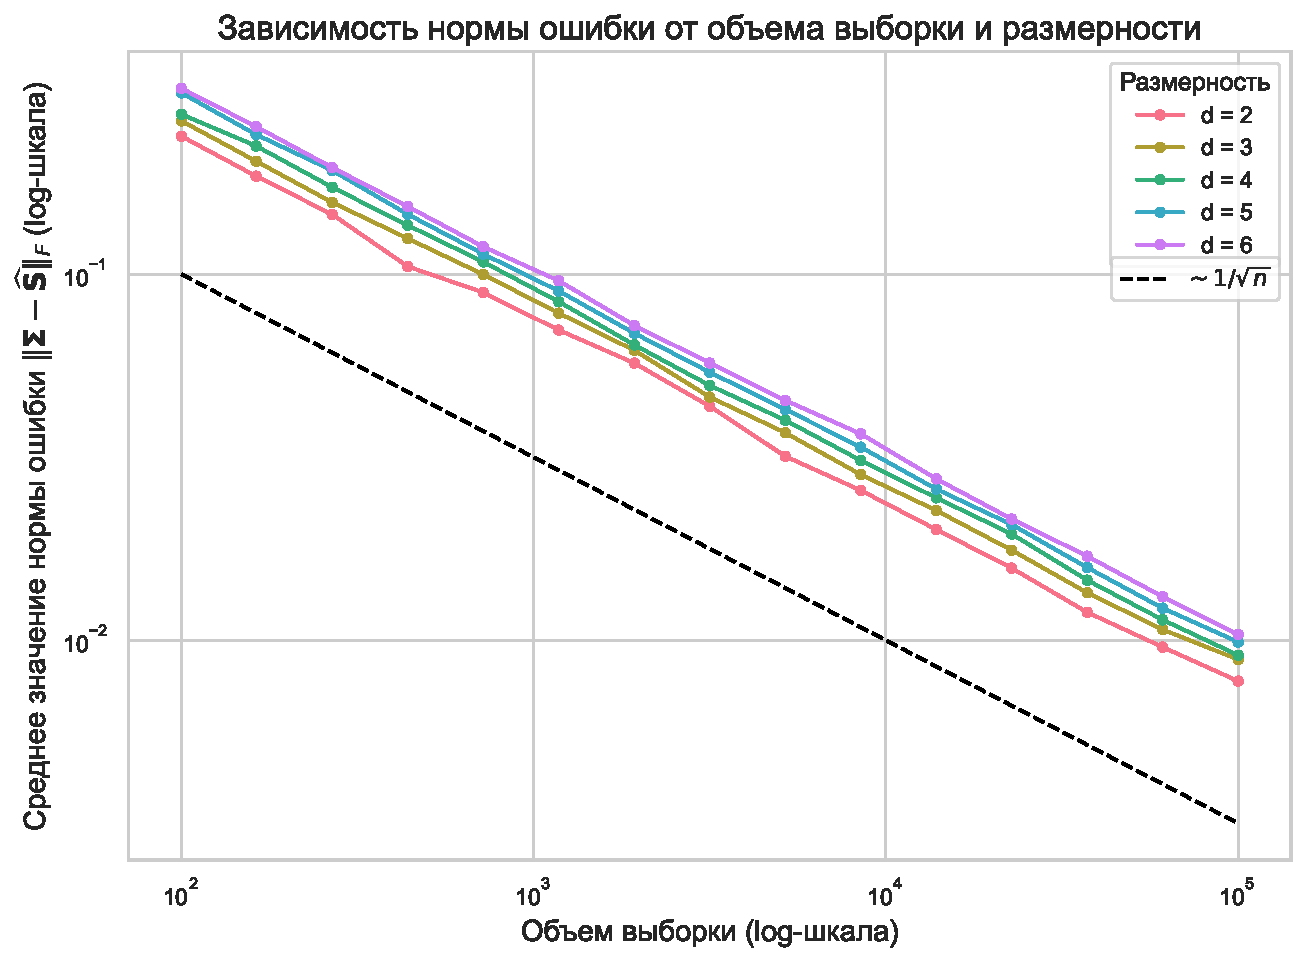
\includegraphics[width=0.95\textwidth]{covariance_consistency_v2.pdf}
    \caption{Зависимость средней нормы ошибки $\|\widehat{\mathbf{S}} - \mathbf{S}\|_F$ от объема выборки $n$ и размерности $d$.}
    \label{fig:consistency}
\end{figure}

\subsection*{Анализ робастности метода ARR-GK}

Во втором эксперименте оценивалась устойчивость метода к добавлению точки-выброса с определенным весом. Сравнение ARR-GK проводилось с классической выборочной ковариационной матрицей на выборке из нормального распределения ($d=3, n=1000$) с истиной ковариационной матрицей \eqref{eq:experimentmatrix} при наличии от 0\% до 25\% выбросов. Для каждой выборки выполнялось $200$ независимых моделирований и рассчитывалась средняя ошибка.

Во втором эксперименте исследовалась устойчивость метода ARR-GK к наличию выбросов. Сравнение проводилось с классической выборочной ковариационной матрицей на выборках из нормального распределения ($d=3$, $n=1000$) с ковариационной матрицей~\eqref{eq:experimentmatrix}.

Для моделирования выбросов часть наблюдений заменялась фиксированной точкой-выбросом, а доля таких наблюдений варьировалась от $0\%$ до $25\%$. Для каждого случая проводилось $200$ независимых моделирований, после чего вычислялась средняя ошибка оценки матрицы разброса.


% Во втором эксперименте исследовалась устойчивость алгоритма ARR-GK к наличию выбросов. Для сравнения рассматривалась классическая выборочная ковариационная матрица.

% Эксперимент проводился на выборках объема $n=1000$ из трехмерного нормального распределения с коррелированными координатами. После генерации выборки часть наблюдений заменялась фиксированной точкой-выбросом большого масштаба. Доля выбросов изменялась от $0\%$ до $25\%$. Для каждой выборки  выполнялось $200$ независимых моделирований.


\begin{figure}[h!]
    \centering
    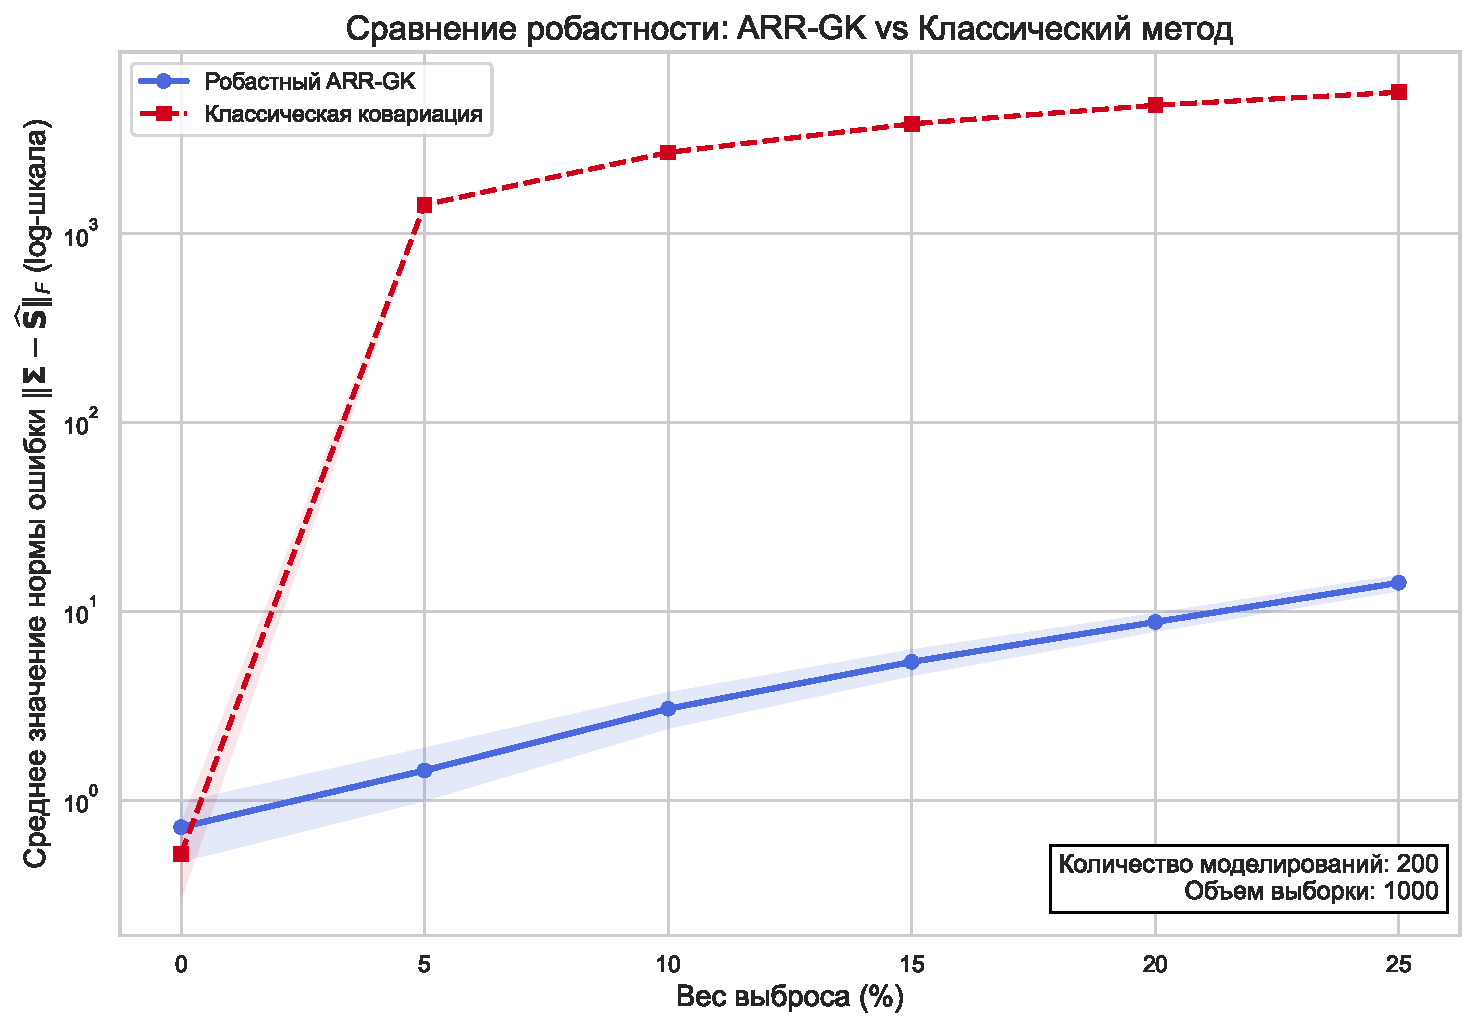
\includegraphics[width=0.9\textwidth]{robustness_comparison_log.pdf}
    \caption{Сравнение робастности ARR-GK и классической ковариационной матрицы при различном весе выбросов.}
    \label{fig:robustness}
\end{figure}

Результаты эксперимента представлены на Рисунке~\ref{fig:robustness}. Видно, что ошибка классической ковариационной матрицы резко возрастает уже при небольшом количестве выбросов. При добавлении $5\%$ выбросов значение ошибки увеличивается на несколько порядков, а дальнейшее увеличение доли выбросов приводит к еще большему ухудшению качества оценки.

В отличие от классического метода, алгоритм ARR-GK демонстрирует существенно более устойчивое поведение. Несмотря на постепенный рост ошибки при увеличении доли выбросов, изменение происходит значительно медленнее, а сама ошибка остается на сравнительно небольшом уровне даже при наличии большого числа выбросов.

Таким образом, проведённый эксперимент показывает, что алгоритм ARR-GK сохраняет устойчивость к выбросам значительно лучше классической выборочной ковариационной матрицы. При увеличении доли выбросов ошибка оценки возрастает существенно медленнее, что экспериментально подтверждает робастность предложенного алгоритма.

\subsection*{Сравнительный анализ ARR-GK с методами GK и F-MCD}

Заключительный эксперимент был направлен на сравнение ARR-GK с базовым методом Гнанадесикана-Кеттеринга (GK) и классическим робастным методом Fast-MCD в различных сценариях.

\textbf{Сравнение на выборке из нормального распределения}

\begin{figure}[h!]
    \centering
    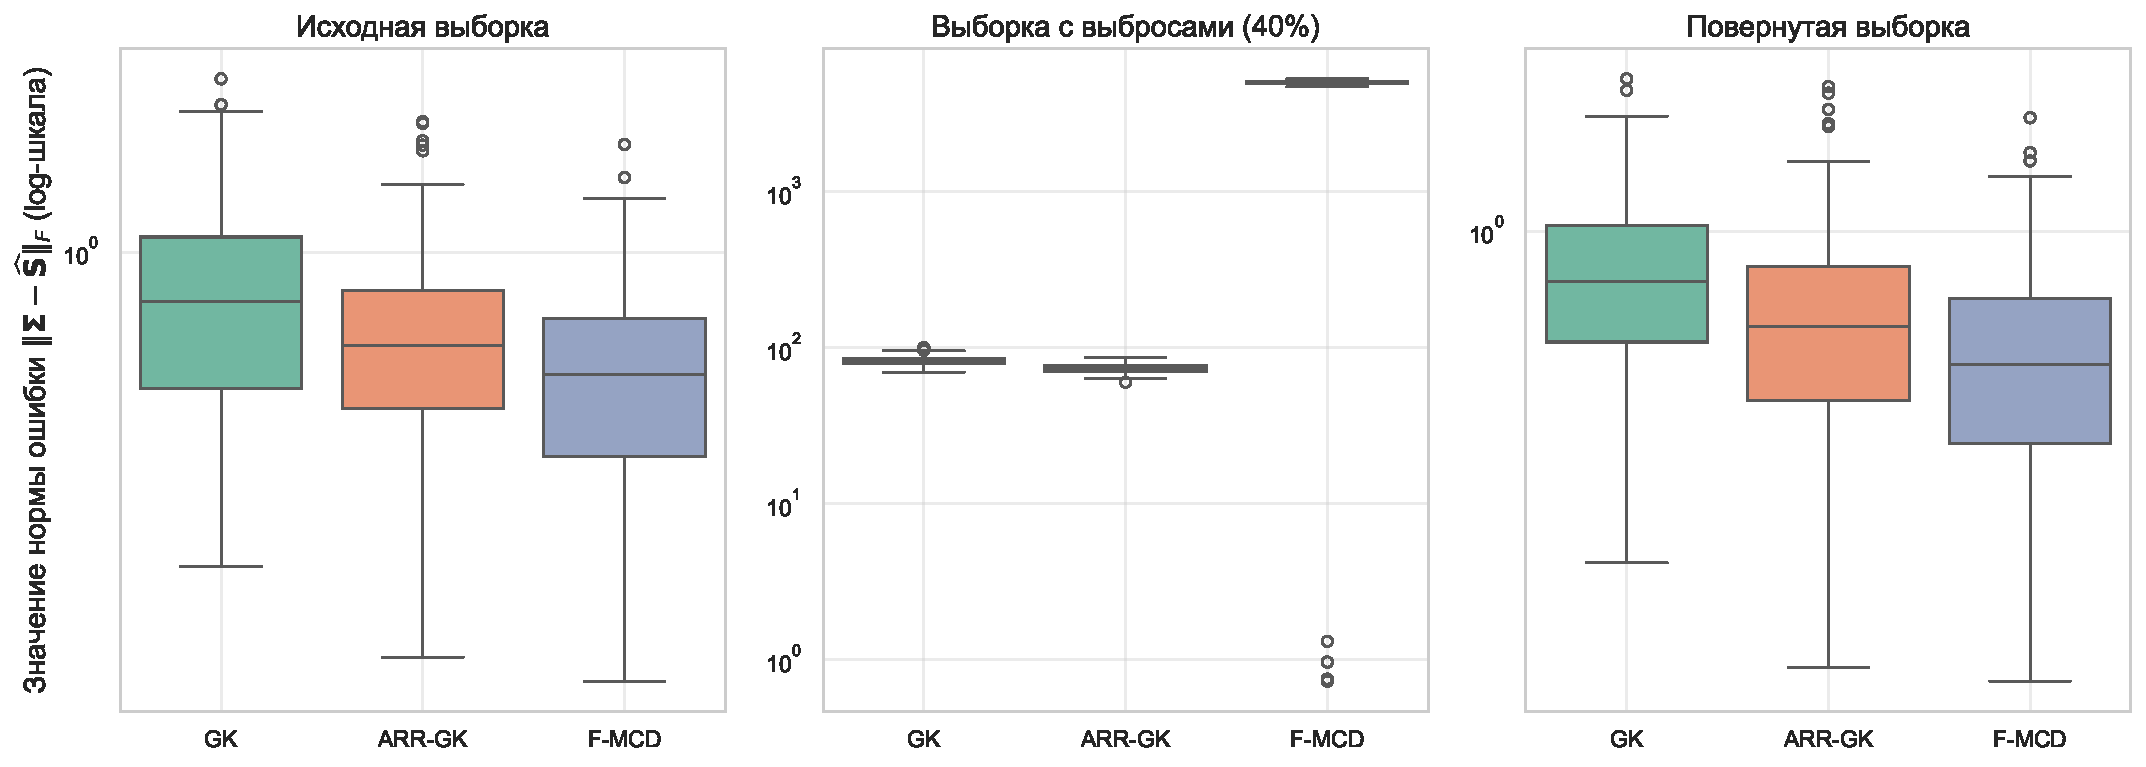
\includegraphics[width=1\textwidth]{comparison_GK_ARR_FMCD.pdf}
    \caption{Распределение нормы ошибки для алгоритмов GK, ARR-GK и F-MCD в различных условиях.}
    \label{fig:comparison_methods}
\end{figure}

На Рисунке~\ref{fig:comparison_methods} представлены результаты сравнения методов GK, ARR-GK и F-MCD для трех различных сценариев: исходной выборки, выборки с $40\%$ выбросов и повернутой выборки.
\begin{enumerate}
    \item \textbf{Исходная выборка:} Для исходной выборки все три метода демонстрируют сопоставимый уровень ошибки. При этом метод F-MCD показывает немного меньшую медианную ошибку и меньший разброс оценок по сравнению с GK и ARR-GK.\vspace{-2ex}
    \item \textbf{Выборка с выбросами (40\%):} В случае выборки с $40\%$ выбросов методы GK и ARR-GK сохраняют устойчивое поведение и дают близкие результаты, тогда как для метода F-MCD наблюдается существенное увеличение ошибки. Это связано с тем, что доля выбросов оказывается близкой к предельному уровню устойчивости метода MCD.\vspace{-2ex}
    \item \textbf{Повернутая выборка:} Для повернутой выборки метод GK демонстрирует увеличение разброса ошибок, тогда как ARR-GK сохраняет более стабильное поведение. При этом метод F-MCD снова показывает наименьшую медианную ошибку среди рассматриваемых алгоритмов. Из-за отсутствия выбросов и простой формы нормального распределения данный сценарий не выявляет особого преимущества ARR-GK перед базовым методом GK. Для того, чтобы продемонстрировать преимущество метода ARR-GK перед GK требуется произвести эксперимент с более сложной выборкой.
\end{enumerate}

Таким образом, результаты эксперимента показывают, что алгоритм ARR-GK позволяет уменьшить чувствительность метода GK к поворотам выборки, сохраняя при этом робастность при наличии большого числа выбросов.

\vspace{1.5ex}

\textbf{Сравнение на несимметричной выборке}

Чтобы показать, что алгоритм GK не устойчив относительно вращений, в отличие от ARR-GK, рассмотрим следующий пример. 

Промоделируем $n=1000$ случайных трехмерных векторов, компоненты которых являются независимыми реализациями экспоненциально распределенной случайной величины с параметром $\lambda=1$, центрированной таким образом, чтобы распределение имело нулевое математическое ожидание и единичную дисперсию.

Далее применим к выборке два линейных преобразования $\mathbf{U}_1$ и $\mathbf{U}_2$, причем $\mathbf{U}_2$ получается из $\mathbf{U}_1$ ортогональным преобразованием:
\begin{equation*}
\mathbf{U}_1 = \begin{pmatrix}
-0{,}707 & -0{,}707 & -1{,}000 \\
-0{,}060 & -1{,}944 & 0{,}467 \\
-2{,}631 & -0{,}161 & 1{,}025
\end{pmatrix}, \quad
\mathbf{U}_2 = \begin{pmatrix}
1{,}414 & 0{,}000 & 0{,}000 \\
0{,}672 & 1{,}884 & 0{,}000 \\
0{,}672 & 0{,}265 & 2{,}735
\end{pmatrix}.
\end{equation*}

Для полученных выборок были применены алгоритмы GK, ARR-GK и F-MCD. Результаты представлены на Рисунке~\ref{fig:comparison_methods_nonnorm}.

Из Рисунка~\ref{fig:comparison_methods_nonnorm} видно, что для исходной выборки методы GK и ARR-GK показывают сопоставимые результаты. Однако после поворота выборки ошибка метода GK существенно возрастает, тогда как качество оценки ARR-GK практически не изменяется. Это экспериментально подтверждает устойчивость предложенного алгоритма относительно вращений выборки.

При этом метод F-MCD в данном эксперименте показывает более высокую ошибку по сравнению с ARR-GK, что особенно заметно для несимметричного распределения.

\begin{figure}[h!]
    \centering
    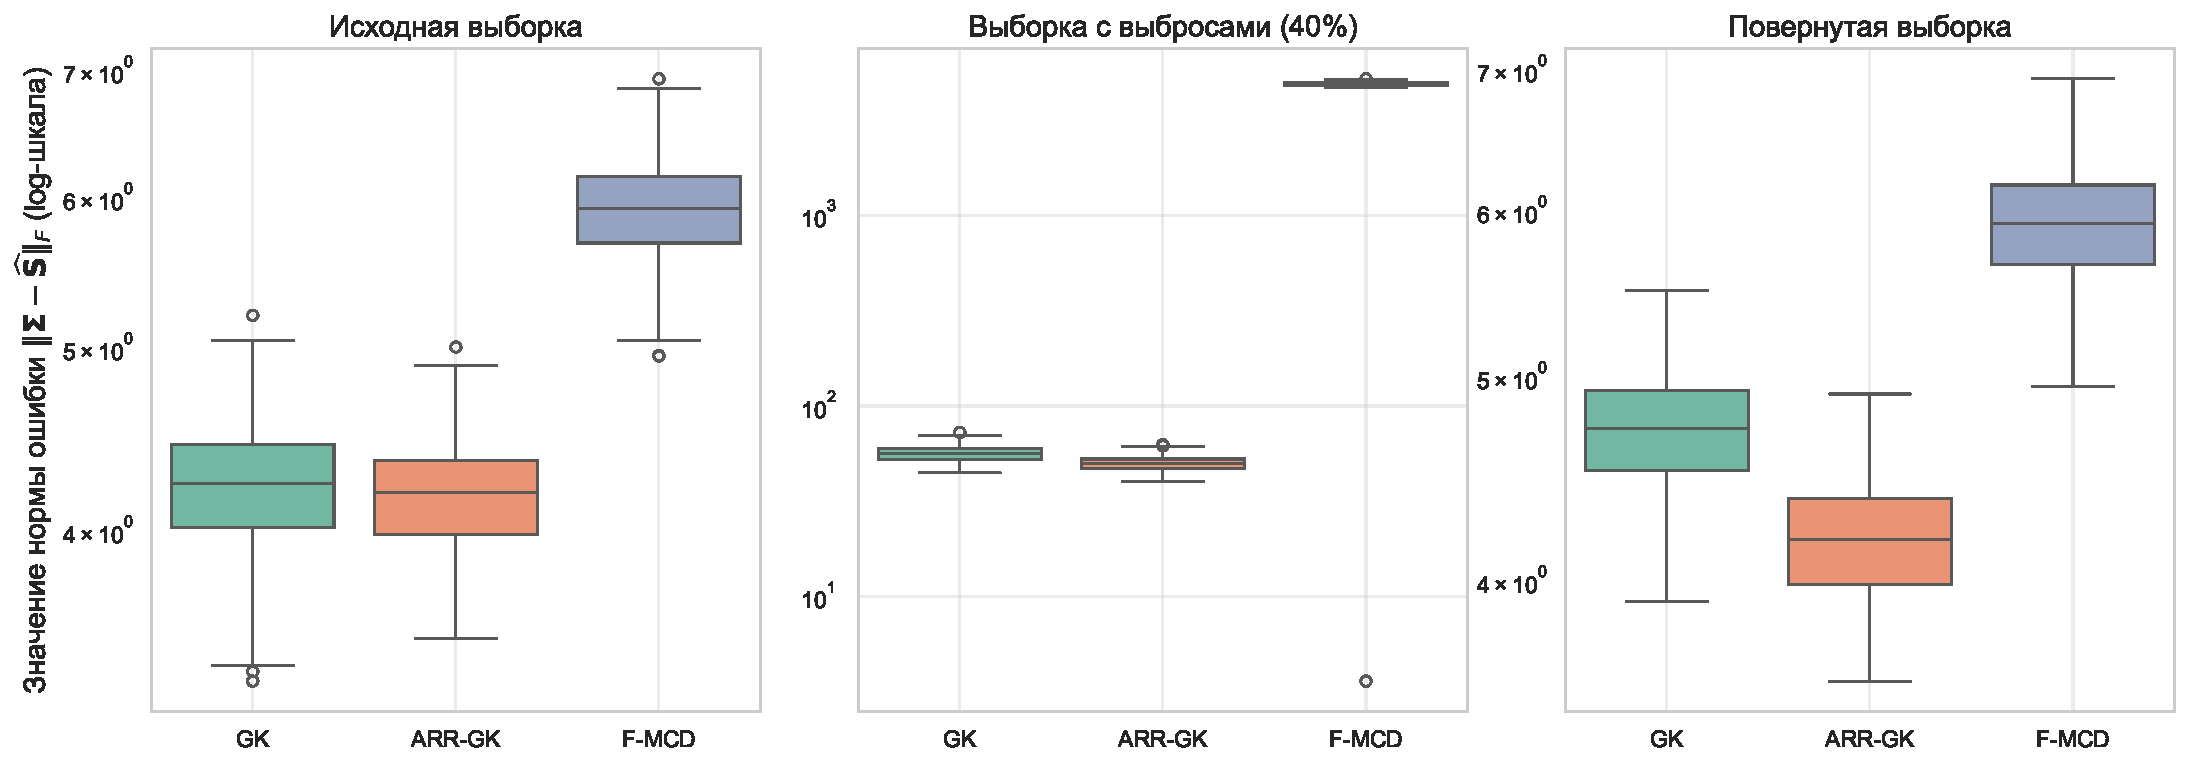
\includegraphics[width=1\textwidth]{comparison_GK_ARR_FMCD_nonnorm.pdf}
    \caption{Распределение нормы ошибки для алгоритмов GK, ARR-GK и F-MCD в различных условиях для исходной выборки (преобразование $\mathbf{U}_1$) и повернутой (преобразование $\mathbf{U}_2$).}
    \label{fig:comparison_methods_nonnorm}
\end{figure}

\vspace{1ex}

Таким образом, проведенные эксперименты показывают, что алгоритм ARR-GK сочетает вычислительную устойчивость метода GK с эквивариантностью относительно вращений. Кроме того, метод сохраняет робастность при наличии выбросов и демонстрирует более стабильное поведение по сравнению с классическим подходом GK на несимметричных распределениях.
